\section{Deep Learning}
Neural networks are heavily researched for numerous applications and they are loosely
based on the way a brain functions. The basic model a \ac{nn} consist of inputs, outputs
and a connecting layer of neurons. This chapter introduces the basic concepts behind
general deep neural networks, convolutional neural networks and stacked denoising
autoencoders.~\ref{ssec:dldnn} and~\ref{ssec:dlcnn} are based on the book Deep Learning by
Goodfellow et.~al.~\cite{DEEP_LEARNING}.

\subsection{Deep neural networks}\label{ssec:dldnn}

A \ac{dnn} is commonly defined as a \ac{nn} that has a \textbf{visible} input and
output layer with several \textbf{hidden layers} between them. The distinction between
visible and hidden layers is important because training of the network only evaluates
the output layer's performance. During training, a \textbf{learning algorithm} optimizes
the individual hidden layers to best approximate the desired output of the whole network.

The input layer takes in the data to be processed, which typically means a vector of
color values in the case of object tracking. These are then processed by the hidden
layers and finally the output layer produces the target's position in the frame. These
models usually come in the form of a \textbf{feedforward neural network} or
\textbf{\ac{mlp}}. The name comes from the fact that information flows from the input
through computations to the output with no \textbf{feedback} connections.

In \ac{nn}s, each layer consist of several \textbf{units} with an activation function
and a weight for each of its input connections. A bias-term can also be defined for
each unit. The weights of a layer are commonly represented by a matrix by which the
input-vector is multiplied. Units in a layer also have a common activation function,
which is fed by the sum of its weighted inputs in addition to the possible bias, and
the result is output to the next layer alongside the layers other units' outputs.
The \textbf{\ac{relu}} is a commonly used unit type, which is defined by the activation
function $g (z) = \max\{0,z\}$. It provides a nonlinear transformation while being
comparable to linear models in terms of generalizing well and being easy to optimize.

\begin{figure}[H]
\centering
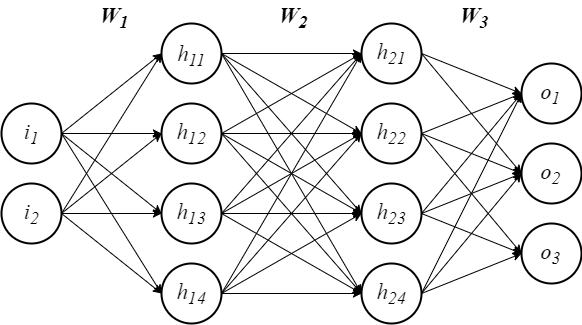
\includegraphics[width=0.75\textwidth]{dnn}
\caption{A fully connected network with two inputs \textit{i}, two hidden layers of
         four units \textit{h} and three outputs \textit{o}. Each set of connections
         is represented by a weight matrix \textbf{W} which indicates mapping from one
         layer to another. Excluding the input, all layers also have an activation
         function and their units can be assigned individual weights.}
\end{figure}

Before training, the weights of a \ac{mlp} are initialized to small random values and 
biases to zero or small positive values. Then an algorithm called \textbf{stochastic
gradient descent} is commonly applied alongside a training dataset. The basic procedure
is to calculate the error of the netwok's output values compared to the desired ones 
using a \textbf{loss function}. The function's gradient can then be calculated for
example by \textbf{back-porpagation}, which feeds the errors back through the network
to assign a contribution value to each unit. These values are then used to calculate
the gradient of the loss function relative to the weights. Each weight is adjusted
slightly to the opposite sign to minimize the loss function.

\subsection{Convolutional neural networks}\label{ssec:dlcnn}

A \ac{cnn} is simply a \ac{nn} that uses convolution instead of general matrix
multiplication in at least one of its layers. The main benefits of convolution in \ac{nn}s
are that it's dramatically more efficient in terms of memory requirements, it reduces
the amount of computation needed and it makes it possible to work with variable input
sizes.

A typical convolutional layer consists of three stages: a convolution stage, detector
stage and pooling stage. These can be implemented by individual layers. First, a
\textbf{kernel} is applied to the input data in positions separated by a stepsize. This
means that a linear activation function is fed by the matrix product of the input location
and the kernel's weight matrix. In the detector stage, the results are then run through
a non-linear activation, for example a \ac{relu}. Finally, a \textbf{pooling function}
is used to combine the results of multiple nearby outputs as the final output.

\begin{figure}[H]
\centering
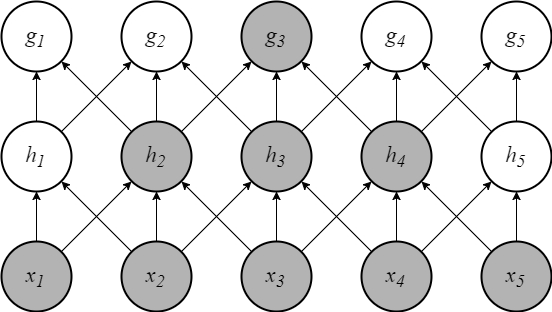
\includegraphics[width=0.75\textwidth]{cnn}
\caption*{Source: Recreated fig. 9.4 from Deep Learing~\cite{DEEP_LEARNING}}
\caption{Deeper layers in a convolutional network are connected to a larger window of the
         input data than shallow layers. This means that deeper layers can be indirectly
         connected to most or all of the input data even though their direct connections
         are sparse.~\cite{DEEP_LEARNING}}
\end{figure}

\subsection{Stacked denoising autoencoders}
Denoising autoencoders are trained to encode a corrupted version of the input to a
hidden representation and decode that to useful features of the clean input. A stacked
denoising autoencoder is simply a sequence of denoising autoencoders trained this way.
Corrupted input is only used to train the individual layers to find useful features
as a trained \ac{sdae} works on clean input.~\cite{SDAE}
\authorcomment{motivation for using sdaes?}
